\documentclass[letterpaper,11pt]{article}
\oddsidemargin -1.0cm \textwidth 17.5cm

\usepackage[utf8]{inputenc}
\usepackage[activeacute,spanish, es-lcroman]{babel}
\decimalpoint
\usepackage{amsfonts,setspace}
\usepackage{amsmath}
\usepackage{amssymb, amsmath, amsthm}
\usepackage{comment}
\usepackage{float}
\usepackage{amssymb}
\usepackage{dsfont}
\usepackage{anysize}
\usepackage{multicol}
\usepackage{enumerate}
\usepackage{graphicx}
\usepackage[left=1.5cm,top=2cm,right=1.5cm, bottom=1.7cm]{geometry}
\setlength\headheight{1.5em} 
\usepackage{fancyhdr}
\usepackage{multicol}
\usepackage{hyperref}
\usepackage{wrapfig}
\usepackage{subcaption}
\usepackage{siunitx}
\usepackage{cancel}
\usepackage{mdwlist}
\usepackage{svg}
\pagestyle{fancy}
\fancyhf{}
\renewcommand{\labelenumi}{\normalsize\bfseries P\arabic{enumi}.}
\renewcommand{\labelenumii}{\normalsize\bfseries (\alph{enumii})}
\renewcommand{\labelenumiii}{\normalsize\bfseries \roman{enumiii})}


\begin{document}

\fancyhead[L]{\itshape{Facultad de Ciencias F\'isicas y Matem\'aticas}}
\fancyhead[R]{\itshape{Universidad de Chile}}
\rfoot[]{pág. \thepage}

\begin{minipage}{11.5cm}
    \begin{flushleft}
        \hspace*{-0.6cm}\textbf{FI1100 Introducción a la Física Moderna}\\
        \hspace*{-0.6cm}\textbf{Tutor:} Alejandro Cartes
    \end{flushleft}
\end{minipage}

\begin{picture}(2,3)
    \put(366, -10){
\includegraphics[scale=0.9]{Imágenes/logo/dfi-fcfm.pdf}}
\end{picture}

\begin{center}
	\LARGE\textbf{Estudiatón C3}\\
	\Large{Ondas acústicas, Óptica Ondulatoria e Intro. QM}
\end{center}

\vspace{-1cm}
\begin{enumerate}\setlength{\itemsep}{0.4cm}

\item[]


\rfoot[]{pág. \thepage}

\item Dos altavoces emiten con la misma frecuencia  y longitud de onda $\lambda=\SI{2.0}{\m}$. Estos se encuentran separados por una distancia $d = \SI{6.0}{\m}$.
Una persona se encuentra a $\ell = \SI{8.0}{\m}$ frente al altavoz derecho (Considere a la persona como un punto).

\begin{enumerate}
    \item Calcule la distancia que debe recorrer la onda generada por cada altavoz hasta la persona.

    \item ¿Qué tipo de interferencia sufrirán las ondas en la posición de la persona?.

    \item Siguiendo el problema anterior, luego de un tiempo la persona ya se encuentra agotada del ruido (o silencio) y solo quiere estar en un lugar silencioso (o ruidoso).
Considerando que la persona se quiere mover lo menos posible y solo alejándose del altavoz derecho. ¿Cuanto debe moverse para cambiar la situación anterior?.
\end{enumerate}

\begin{minipage}{0.65\linewidth}
    \item \textbf{[P3-C1 2023-1]} Un diapasón es una varilla metálica en forma de U. El sonido emitido por el diapasón contiene una sola frecuencia que viene grabada en este dispositivo y es igual a $\SI{384}{\Hz}$. El diapasón puede usarse para poder encontrar la velocidad del sonido en una columna de aire, para esto, se busca la frecuencia en la que se produce resonancia (cuando la frecuencia del diapasón coincide con algún modo normal de la columna de aire). Considere el esquema mostrado en la figura, en donde se tiene una columna de aire en un tubo de vidrio con un extremo abierto en la parte superior y cerrado en el otro lado mediante un pistón móvil. Cuando el pistón está a $\SI{22.8}{\cm}$ del extremo abierto se escucha resonando y, una vez más, cuando está a $\SI{68.3}{\cm}$ del extremo abierto.
\end{minipage}
\hfill
\begin{minipage}{0.3\linewidth}
    \begin{figure}[H]
        \centering
        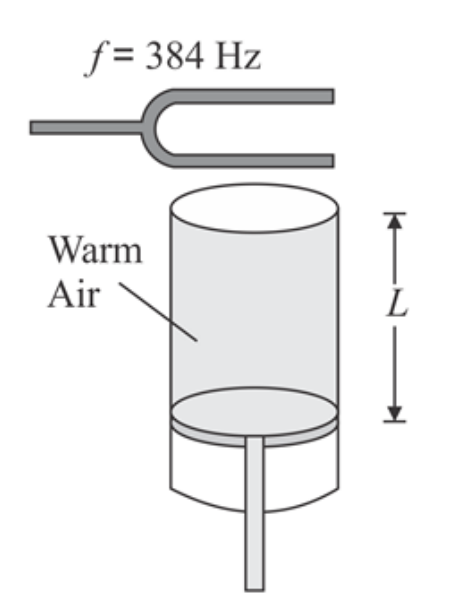
\includegraphics[width=0.9\linewidth]{Imágenes/tutorias/image.png}
    \end{figure}
\end{minipage}
\begin{enumerate}
    \item ¿Qué rapidez de sonido se implica con estos datos?
    \item ¿A qué distancia $L$ del extremo abierto estará el pistón cuando se escuche la siguiente resonancia?
\end{enumerate}


\item \textbf{[P2-C3 2020-2]} Se realiza un experimento de doble rendija usando un láser de He-Ne ($\lambda = \SI{633}{\nm}$). Luego, se coloca un placa muy delgada de vidrio ($n = 1.5$) sobre una de las ranuras. Se observa que el punto central en la pantalla está ahora ocupado por la que había sido la franja oscura correspondiente a $m = 10$. ¿Cuán grueso es el vidrio?
Considere que la pantalla está ubicada muy lejos, de manera que vale la aproximación paraxial (todos los ángulos son muy pequeños).

\item Una luz con una longitud de onda de $\SI{580}{\nm}$ incide sobre una rendija con un ancho de $\SI{0.300}{\mm}$. La pantalla de observación está a $\SI{2.00}{m}$ de la rendija. Determine las posiciones de las primeras franjas oscuras, así como el ancho de la franja central brillante.


\item Vamos a demostrar para un átomo hidrogenoide que $E~\propto~n^{-2}$, para ello:
\begin{enumerate}
    \item Recordando que la fuerza electrostática es de la forma
    $$\left|{\vec{F}}\right| = \frac{K q_1 q_2}{r^2} $$
    
    Utilizando además que $L = n\hbar$, obtenga una expresión para el radio de órbita de un electrón.
    
    \item Recordando que la energía potencial para la fuerza de Coulomb se define como
    $$ U = -\frac{Kq_1q_2}{r}$$
    
    Determine una expresión para la energía.
    
    \item Con esto demuestre que para dos niveles de energía $n, m$ (con $m>n$) se tiene que la transición de un estado de mayor energía a uno de menor energía cumple:
    $$\frac{1}{\lambda} = Z^2 R_H\left(\frac{1}{n^2}-\frac{1}{m^2}\right)$$
\end{enumerate}


\item Considere un átomo de berilio (Z=4) al cual se le quitan tres electrones. Para este átomo:
\begin{enumerate}
    \item ¿Cuál es la energía fundamental? Compare con el átomo de Hidrógeno.
    \item ¿Cuál es la energía de ionización? Compare con el átomo de Hidrógeno.
    \item Para el Hidrógeno se tiene que la longitud de onda emitida por un fotón debido a una transición de n=2 a n=1 es 122 nm. ¿Cuál será la longitud de onda emitida de un fotón debido a esta misma transición?
    
    \item Para un valor dado de $n$, compare el radio de órbita de un electrón en este átomo con el hidrógeno.
\end{enumerate}

\end{enumerate}
\end{document}

% Para imágenes vectoriales -> el texto tiene que estar en LaTeX
% \begin{figure}[htbp]
%   \centering
%   \svgpath{../Imagenes/ejercicios}  -> .. irse pa'trás 
%   \includesvg{ej5.svg}
% \end{figure}
